\chapter{Synthesis}
\label{synthesis}

%% Start the actual chapter on a new page.
\newpage

% De Intro en Synthese hoeven van mij geen lange verhalen te zijn, maar moeten het werk dat in 
% de hoofdstukken staat in de wetenschappelijke context plaatsen. Hier moeten dus de praktische 
% vragen worden gesteld:  
% wat we hier dan mee kunnen (Synthese). .... Je kunt ook aangeven welke opties in 
% BEAST2 nog niet zijn geimplementeerd (en waarom), daarbij in wat meer detail aangevend wat 
% die opties inhouden (bijv. partities, *BEAST).





\section{Today}

\noindent

\dropcap{T}{his} thesis demonstrates the error we make in 
inferring our phylogenies, for two speciation models.
However, there are many more speciation models.

Take, for examples the genus of \textit{setophaga}.
Figure \ref{fig:setophaga} shows a phylogeny is 
Taking a closer look at the number of lineages through time,
we can see that this number increases less and less through time.

\begin{figure}[H]


  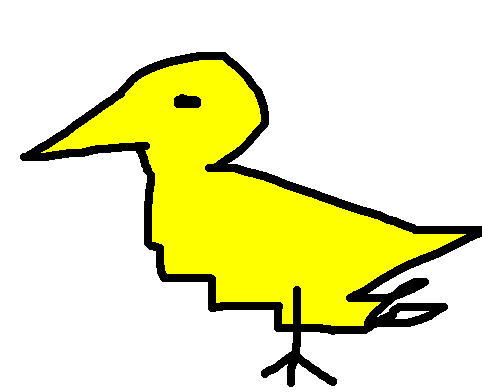
\includegraphics[width=0.3\textwidth]{setophaga.png}
  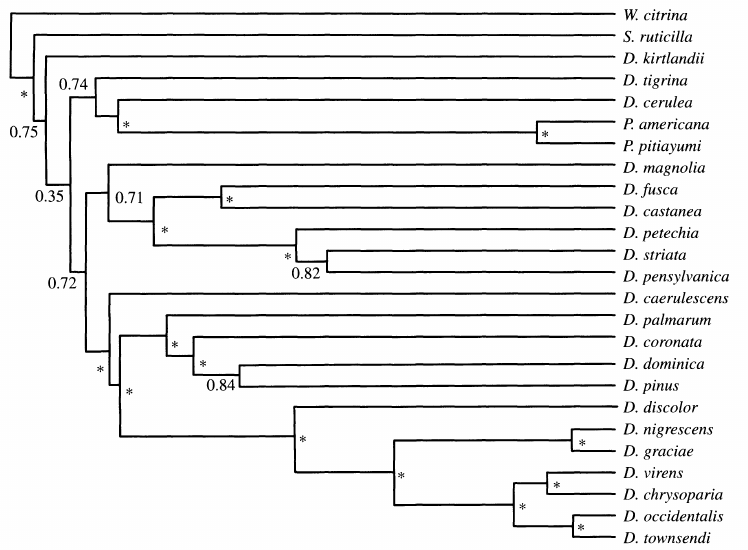
\includegraphics[width=0.3\textwidth]{rabosky_lovette_2008_setophaga_phylogeny.png}
  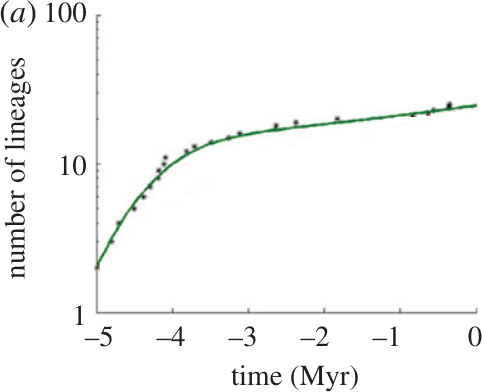
\includegraphics[width=0.3\textwidth]{etienne_et_al_2011_fig_3_a.png}
  \caption{
    A \textit{setophaga somethingus} of the genus \textit{setophaga}.
    A \textit{setophaga} phylogeny, from Rakosky and Lovette (2008).
    The number of \textit{setophaga} species through time, adapted from Etienne et al 2011
  }
  \label{fig:setophaga}
\end{figure}



\dropcap{O}{nce} upon a time, a scientific conference on speciation was
organised. Ariel, a PhD, was there. 
Ariel has the feeling that standard phylogenetic models
oversimplify. Standard phylogenetic models show
an exponential growth (or decline) in the number of taxa.
Due to this, these models predict that after an
infinite amount of time, there will be zero or an infinite amount of species.
Ariel thinks this is unrealistic and is a proponent of the DDD 
model (Etienne & Haegeman, 20??), in which there is an upper limit (a
'carrying capacity') on the number of species. Ariel wonders what
error we have made in our phylogentic inference due to this.

Jasmine, also a PhD, was also at that same conference. Jasmine, who
has some field experience in working with cichlids, 
has the feeling that standard phylogenetic models
oversimplify. Standard phylogenetic models assume that speciation and
extinction rates are constant through time. 
Jasmine thinks this is unrealistic, as she thinks 
speciation is dependent on the traits (opsins, jaw) that species have.
Due to this, Jasmine is a proponent of the trait-dependent
diversification model (?Madisson, 20??). Jasmine wonders what
error we have made in our phylogentic inference due to this.

Luckily for them, Ariel and Jasmine met Belle at that conference.





thesis resulted in four articles,
of which two are methodological and two are illustrations
of applying it. 

What can we do with it?


\subsection{Chapter 2: \texttt{babette}}

Chapter 2 shows the flexibility of \verb;babette;, where this whole thesis
shows its robustness: all the following chapters use \verb;babette; to
do Bayesian inference in a scripted way. Also, \verb;babette; has passed
the stringent code peer-review by rOpenSci, which is another indicator of 
its quality.

Nevertheless, there is one trait of recognition of \verb;babette; missing:
it has zero citations up until now, when excluding the articles in this 
thesis. We think the reason for it is that \verb;babette; is
not on CRAN yet. There are multiple reasons why this is the case:
First, \verb;babette; consists out of five packages. Three out of these
five packages have a dependency on the others. Therefore, the packages can
be submitted in sequence only. Second, \verb;babette; has remained in active 
development since its conception. There was a prioritization of 
fixing a known bug and adding a vital new feature over 
pushing \verb;babette; to CRAN and hurting users. Third, \verb;babette;
only supports a certain percentage of BEAST2 use cases, which are the
use cases needed for this thesis. 

So although \verb;babette; is still underappreciated, it has only gotten
better before it will get the attention it deserves. 
For example, after the publication of its article, 
a feature has been added to run \verb;babette; in parallel
jobs on the Groningen computer cluster, paving the way for heavy-duty 
usage. Without this new feature, chapters 4 and 5 would have been
impossible to complete.

\subsection{Chapter 3: \texttt{pirouette}}

Chapter 3 shows the usage of \verb;pirouette;, a tool to measure the
impact/relevance of a novel tree prior. \verb;pirouette; is flexible and
robust enough to be used in the next two chapters. Also, when averaging
out the stochasticity, \verb;pirouette; works as expected, successfully
quantifying the impact that a novel tree prior has.

\verb;pirouette; provides a good first step to determine 
if a novel tree prior is relevant in a Bayesian analysis:
instead of following intuition, \verb;pirouette; expresses 
the added value of a new tree prior in numbers. The second step,
however, is still missing: a clear-cut interpretation of these numbers.

 * How often are new tree priors created?
 * Isn't it easier to write the new tree prior in BEAST2 to assess its
   relevance?
 * Pipeline is complex:
   * Effect of alignment's site and clock model
   * Effect of error function: nLTT, or gamma statistic or 
 * Quantification still has to interpretated

 * pirouette only uses an alignment and discards other data

\subsection{Chapter 4: \texttt{razzo}}

Chapter 4 shows the error in a Bayesian inference on
phylogenies in which speciation co-occurs, when using standard
tree priors that do not allow for co-occuring speciation.
Me and my co-author quantify the errors made under a wide range
of parameter settings. The more frequent to co-occurance of speciation,
[it is expected] the larger the error. 
[it is yet unknown if that error is big compared to the background noise]

 * More fine-grained parameter space, but why?

\subsection{Chapter 5: \texttt{raket}}

Chapter 5 shows the error in a Bayesian inference on
phylogenies in which speciation takes time, when using standard
tree priors that do not allow for speciation taking time.
I quantify the errors made under a wide range
of parameter settings. The longer speciation takes, [it is expected] the larger the error. 
[it is yet unknown if that error is big compared to the background noise]
The effect of sampling a representative incipient species to create
a species tree are [expected to be] small.

This thesis gives the field of phylogenetics tools and examples of
how to quantify the effect of a tree prior on Bayesian inference.
It will help research find the border between when speciation models are
simple enough, yet not too simple. As all articles within this thesis,
this thesis itself and all its source code is free (as in freedom),
there is little in the way of this research contributing to the field. 

% Het hoofdstuk conclusion is meer een synthese of discussie. Een
% outlook naar de toekomst. Hier kun je ook ideeen kwijt die niet in de
% hoofdstukken terecht zijn gekomen.

\section{Future}

 * Improve babette
 * Apply pirouette to standard models
   * Measure effect of n taxa
   * Measure effect of DNA sequence length
   * Measure effect of stochasticity in alignment
   * Measure effect of absolute nLTT statistic: squared nLTT, 
     log-transformed nLTT, delta R 
   * Measure effect of more candidates
   * Effect of using the MRCA prior
   * Interpretation of error distributions 
 * Measure impact of MBD prior differently, by adding it to BEAST2
   anyways, then do an MCMC that switch models
 * Measure impact of PBD prior differently, by adding it to BEAST2
   anyways, then do an MCMC that switch models



\references{conclusion}

